% !TeX spellcheck = pl_PL
\documentclass[a4paper,twoside]{article}
\usepackage{polski}
\usepackage[utf8]{inputenc}
\usepackage{graphicx}
\usepackage{amsmath}

\usepackage[unicode, bookmarks=true]{hyperref} %do zakładek
\usepackage{tabto} % do tabulacji
\NumTabs{6} % globalne ustawienie wielkosci tabulacji
\usepackage{array}
\usepackage{multirow}
\usepackage{array}
\usepackage{dcolumn}
\usepackage{bigstrut}
\usepackage{color}
\usepackage[usenames,dvipsnames]{xcolor}
\usepackage{svg}
\usepackage{xfrac}
\usepackage{floatrow}
\usepackage{listings,lstautogobble}

\usepackage{multirow,tabularx}
\newcolumntype{Y}{>{\centering\arraybackslash}X}
\renewcommand{\arraystretch}{2}

% === Reset inkrementacji sekcji przy nowym parcie === %
\usepackage{titlesec}

\makeatletter
\@addtoreset{section}{part}
\makeatother
\titleformat{\part}[display]
{\normalfont\LARGE\bfseries\centering}{}{-60pt}{}

% === Dodanie krpki do sekcji
\titlelabel{\thetitle.\quad}


\setlength{\textheight}{24cm}
\setlength{\textwidth}{15.92cm}
\setlength{\footskip}{10mm}
\setlength{\oddsidemargin}{0mm}
\setlength{\evensidemargin}{0mm}
\setlength{\topmargin}{0mm}
\setlength{\headsep}{5mm}

\setlength{\textfloatsep}{10pt plus 1.0pt minus 2.0pt}

% --- Opcje listingu kodu
\lstset{
	frame=single,
	autogobble=true,
	commentstyle=\ttfamily\itshape\color{gray},
	keywordstyle=\color{blue},
	frameround=ffff,
	rulecolor=\color{black},
	tabsize=4,
	breaklines=true, %
	% --- Polskie znaki w listingu kodu
	literate=%
	{ą}{{\c{a}}}1
	{ć}{{\'c}}1
	{ę}{{\c{e}}}1
	{ł}{{\l{}}}1
	{ń}{{\'n}}1
	{ó}{{\'o}}1
	{ś}{{\'s}}1
	{ź}{{\'z}}1
	{ż}{{\.z}}1
	{Ą}{{\c{A}}}1
	{Ć}{{\'C}}1
	{Ę}{{\c{E}}}1
	{Ł}{{\L{}}}1
	{Ń}{{\'N}}1
	{Ó}{{\'O}}1
	{Ś}{{\'S}}1
	{Ź}{{\'Z}}1
	{Ż}{{\.Z}}1
}
\lstset{
	basicstyle=\ttfamily,
	columns=fullflexible,
	showstringspaces=false,
	commentstyle=\color{gray}\upshape
}


\begin{document}
\bibliographystyle{plain}

	% ************************************************************
	% --- Strona tytułowa
	% ************************************************************
	\begin{titlepage}
		\begin{table}[htbp]
			\centering
			\begin{tabular}{|c|c|c|c|c|c|c|}
				\hline
				\multicolumn{7}{|c|}{\textbf{{\LARGE Projekt programistyczny}}} \bigstrut\\[4pt]
				\hline
				Rok akademicki & Termin & Rodzaj studiów & Kierunek & Prowadzący & Grupa & Sekcja \bigstrut\\
				\hline
				\multicolumn{1}{|c|}{\multirow{2}[4]{*}{{\large 2014/2015}}} & \multicolumn{1}{c|}{{\large Wtorek}} & \multicolumn{1}{c|}{\multirow{2}[4]{*}{{\large SSI}}} & \multicolumn{1}{c|}{\multirow{2}[4]{*}{{\large INF}}} & \multicolumn{1}{c|}{\multirow{2}[4]{*}{\begin{tabular}{@{}c@{}}{\large dr inż.} \\[-9pt] {\large Arkadiusz}\\[-9pt] {\large Biernacki}\end{tabular}}} & \multicolumn{1}{c|}{\multirow{2}[4]{*}{{\large GKiO3}}} & \multicolumn{1}{c|}{\multirow{2}[4]{*}{{\large 1}}} \bigstrut\\
				\cline{2-2}    \multicolumn{1}{|c|}{} & \multicolumn{1}{c|}{{\large 12:45 - 15:00}} & \multicolumn{1}{c|}{} & \multicolumn{1}{c|}{} & \multicolumn{1}{c|}{} & \multicolumn{1}{c|}{} & \multicolumn{1}{c|}{} \bigstrut\\
				\hline
			\end{tabular}%
		\end{table}%
		
		\centering
		
\includegraphics[width=0.6\textwidth]{./images/logo.png}
		\\\vspace{10mm}
		\textbf{{\huge Realizacja wybranego przypadku użycia}}\\\vspace{5mm}
		\textbf{{\Huge Danmaku Shooter}}
		\\
		\vfill
		\begin{flushright}
				{\Large \textbf{Skład sekcji}:}\\
			\begin{tabular}{rr}
				{\Large Buchała} & {\Large Bartłomiej}\\[-3pt]
				{\Large Forczmański} & {\Large Mateusz}\\[-3pt]
				{\Large Motyka} & {\Large Marek}\\[-3pt]
				{\Large Wudecki} & {\Large Wojciech}
			\end{tabular}
		\end{flushright}
	\end{titlepage}

	\part{\huge \textbf{Wybrany diagram przypadku użycia}}
	
	\begin{figure}[h!]
		\hspace{-25mm}
		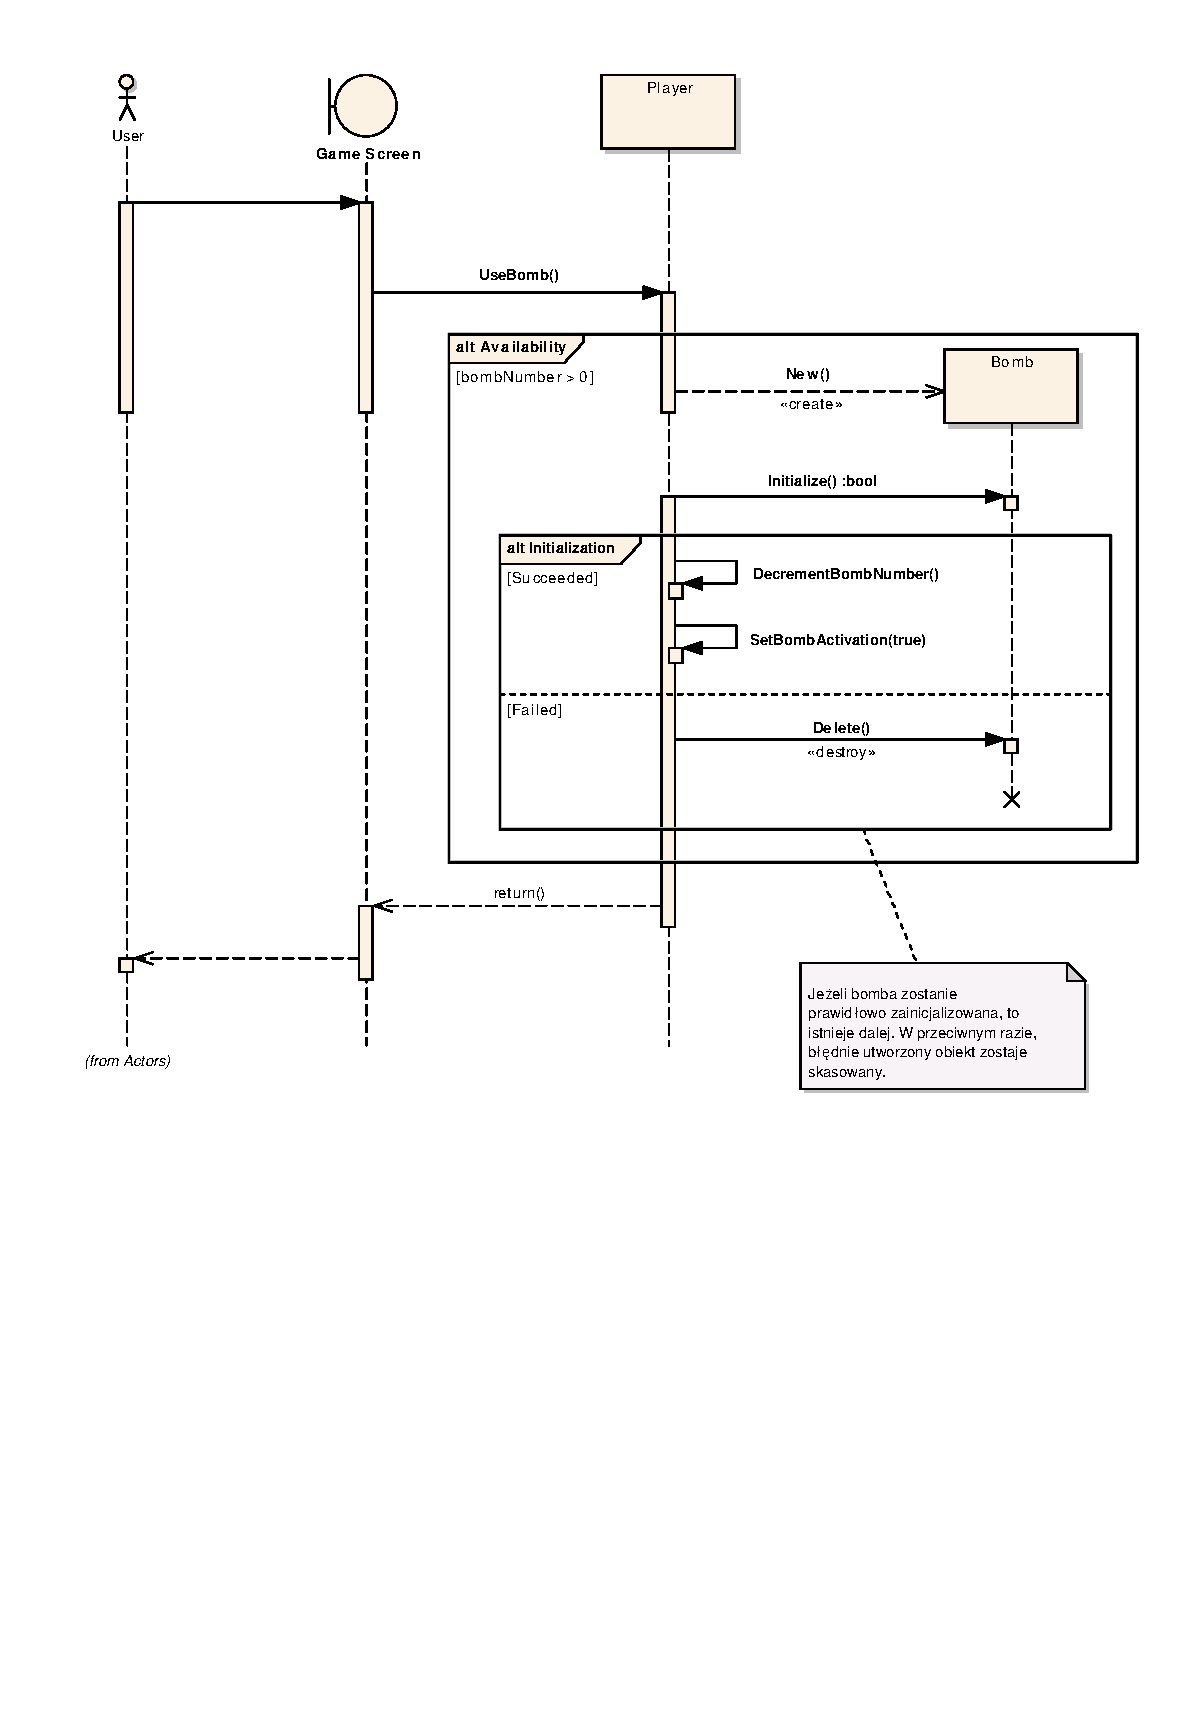
\includegraphics[width=1.15\textwidth, trim={0 10cm 2cm 0}]{./images/Bomba.pdf}
		\caption{{\large Diagram przepływu przypadku użycia bomby}}
	\end{figure}
	
	\newpage
	\part{\huge \textbf{Specyfikacja wewnętrzna}}
		\section{Implementacja uruchomienia bomby}
			\subsection{Wywołanie metody}
				Za interfejs \emph{Game Screen} odpowiada klasa Game. Gdy użytkownik zażyczy sobie włączyć bombę, poniższy fragment kodu zostaje wywołany.
				\begin{lstlisting}[language=C++]
					void Game::Update(float const time)
					{
						if (input->GameKey(GameControl::BOMB))
						{
							if(this->player->UseBomb())
							{
								this->bombBar->DecrementCount();
								this->player->SetIsInvulnerable();
							}
						}
					}
				\end{lstlisting}
				W momencie gdy wykorzystanie bomby się powiedzie, w interfejsie gry zostaje zmniejszony licznik bomb, a sam gracz staje nie się nietykalny i nie można go zranić.
			\subsection{Użycie bomby (funkcja UseBomb())}
				\begin{lstlisting}[language=C++]
					bool Player::UseBomb()
					{
						if (!IsUsingBomb() && _bombCount > 0)	
						{
							_bomb->Launch();
							DecrementBombNumber();
							return true;
						}
						return false;
					}
				\end{lstlisting}
				W funkcji sprawdzana jest dostępność bomby - licznik musi mieć wartość większą od zera oraz bomba nie może być w użyciu (jednocześnie może być uruchomiona tylko jedna). Jeżeli warunek jest spełniony, bomba zostaje uruchomiona. W przeciwnym wypadku nic się nie dzieje.
				\subsubsection{Wystrzelenie bomby (funkcja Launch())}
					W funkcji \textit{Launch}() klasy Bomb następuje zaznaczenie, że bomba jest już aktywowana.
					\begin{lstlisting}[language=C++]
						void Bomb::Launch()
						{
							_elapsedTime = 0;
							SetBombActivation(true);
						};
					\end{lstlisting}
					\begin{lstlisting}[language=C++]
						void Bomb::SetBombActivation(bool activated)
						{
							_activated = activated;
						};
					\end{lstlisting}
					Ideą jest enkapsulacja informacji - gracz wie, ile bomb ma do wykorzystania, z kolei to bomba wie, czy jest w użyciu lub nie.
				\subsubsection{Dekrementacja licznika bomb}
					Ciało funkcji gracza, która zmniejsza liczbę bomb, wygląda następująco:
					\begin{lstlisting}[language=C++]
						void Player::DecrementBombNumber()
						{
							if (_bombCount > 0)
								_bombCount--;
						}
					\end{lstlisting}
			\subsection{Utworzenie bomby}
				Podczas tworzenia gry uległa zmianie konstrukcja obiektu bomby. Ponieważ forma i realizacja bomby, zawsze jest taka sama, aby zmniejszyć liczbę obliczeń i nie ładować tych samych sprajtów, jest ona tworzona tylko raz, podczas uruchamiania gry. Natomiast w trakcie rozgrywki, użytkownik jedynie wczytuje obiekt bomby oraz każe jej realizować tę samą operację wystrzału.\\\\
				Jeżeli podczas uruchamiania gry, bomba (albo inny istotny obiekt) nie zostanie prawidłowo wczytany, gra się nie uruchomi - nie było sensu w tym, żeby gracz uruchamiał niekompletną grę lub w czasie \textit{gameplay}'u istniało niepotrzebnie większe prawdopodobieństwo niepowodzenia uruchomienia któregoś z elementów.\\\\
				Aktualny proces tworzenia obiektu bomby wygląda następująco:
				\begin{enumerate}
					\item W czasie uruchamiania gry, instancja bomby zostaje utworzona poprzez klasę gracza:
					\begin{lstlisting}[language=C++]
					bool Player::InitializeBomb(LPDIRECT3DDEVICE9 device)
					{
						_bomb = BombPtr(new Bomb(&centerPoint));
						return _bomb->Initialize(device);
					};
					\end{lstlisting}
					\item Jeżeli utworzenie bomby się nie powiodło, w klasie gry zostaje wyrzucony wyjątek i inicjalizacja gry kończy się niepowodzeniem:
					\begin{lstlisting}[language=C++]
					bool Game::Initialize()
					{
						try
						{
							if (!this->CreatePlayer())
								throw PlayerInitializationFailedException();
							return true;
						} catch (GameInitializationFailedException & ex)
						{
							ex.ToMessageBox();
							return false;
						}
					}
					\end{lstlisting}
					\begin{lstlisting}[language=C++]
					bool Game::CreatePlayer()
					{
						bool success = true;
						success &= this->player->InitializeBomb(gDevice->device);
						return success;
					}
					\end{lstlisting}
					\item W przypadku niepowodzenia, gra zwraca informację, że nie została poprawnie utworzona, a jej instancja - wraz z jej wszystkimi elementami, w tym bombą - zostaje usunięta.
				\end{enumerate}
			\section{Odwołania do interfejsów}
				\subsection{IDrawable}
					\subsubsection{Opis}
						Klasy implementujące ten interfejs mogą zostać wyświetlone na ekranie gry.
					\subsubsection{Klasy wykorzystujące ten interfejs}
						\begin{itemize}
							\item Sprite
						\end{itemize}
					\subsubsection{Metody interfejsu} Wyświetlenie elementu na ekranie. Funkcja przyjmuje pozycję, gdzie sprajt ma zostać wyświetlony, oraz jego skalę i obrót. Implementacja funkcji musi zapewnić, że sprajt zostanie prawidłowo wyświetlony zgodnie z przekazanymi parametrami.
							\begin{lstlisting}[language=C++]
								virtual void Draw(D3DXVECTOR2 const & position, float scale, float rotation) = 0;
							\end{lstlisting}
					\subsubsection{Fragmenty implementacji}
						\begin{lstlisting}[language=C++]
							class Sprite : public IDrawable
							{
							public:
								void Draw(D3DXVECTOR2 const & position, float scale = 1.0f, float rotation = 0.0f) override;
							};
							
							void Sprite::Draw(D3DXVECTOR2 const & position, float scale, float rotation)
							{
								if (this->sprite && tex)
								{
									this->sprite->Begin(D3DXSPRITE_ALPHABLEND);
									D3DXMATRIX mat;
									D3DXVECTOR2 center2D( position.x + center.x, position.y + center.y );
									D3DXVECTOR3 position3D( position.x, position.y, 0.0f );
									// skalowanie i obrót
									D3DXMatrixTransformation2D( &mat, &center2D, NULL, new D3DXVECTOR2( scale, scale ), &center2D, rotation, NULL );
									this->sprite->SetTransform( &mat );
									this->sprite->Draw(tex[this->currentTex], NULL, NULL, &position3D, this->color);
									this->sprite->End();
								}
							};
						\end{lstlisting}
				\newpage
				\subsection{ITransformable}
					\subsubsection{Opis}
						Klasy implementujące ten interfejs mogą zmieniać swój kształt i pozycję.
					\subsubsection{Klasy wykorzystujące ten interfejs}
						\begin{itemize}
							\item GameObject
							\item Hitbox
							\item Trajectory
						\end{itemize}
					\subsubsection{Metody interfejsu}
					\begin{enumerate}
						\item Przesunięcie całego obiektu zgodnie z przekazanym wektorem.
						\begin{lstlisting}[language=C++]
							virtual void Translate( D3DXVECTOR2 const & translate ) = 0;
						\end{lstlisting}
						\item Proporcjonalne skalowanie obiektu zgodnie z przekazaną skalą.
						\begin{lstlisting}[language=C++]
							virtual void Scale( float const scale ) = 0;
						\end{lstlisting}
						\item Obrót całego obiektu wokół własnego środka o zadany kąt.
						\begin{lstlisting}[language=C++]
							virtual void Rotate( float const theta ) = 0;
						\end{lstlisting}
					\end{enumerate}
					\subsubsection{Fragmenty implementacji}
					\begin{lstlisting}[language=C++]
						class GameObject: public ITransformable
						{
						public:
							void Translate( D3DXVECTOR2 const & dv ) override;
							void Rotate( float const angle ) override;
							void Scale( float const scale ) override;
						};
						void GameObject::Translate( D3DXVECTOR2 const & dv )
						{
							this->position += dv;
						};
						void GameObject::Scale( float const scale )
						{
							this->scale *= scale;
							this->hitbox->Scale( scale );
						};
						void GameObject::Rotate( float const angle )
						{
							this->rotation += angle;
						};
					\end{lstlisting}
				\newpage
				\subsection{IException}
					\subsubsection{Opis}
						Klasy implementujące ten interfejs służą do generowania wyjątków i muszą zostać prawidłowo obsłużone.
					\subsubsection{Klasy wykorzystujące ten interfejs}
					\begin{itemize}
						\item Direct3DInitializationFailedException
						\item FileException
						\item GameInitializationFailedException
						\item GameWindowInitializationFailedException
						\item StageCreationFailedException
					\end{itemize}
					\subsubsection{Metody interfejsu}
					\begin{enumerate}
						\item Zwrócenie komunikatu w postaci łańcucha znakowego.
						\begin{lstlisting}[language=C++]
							virtual std::string ToString() const = 0;
						\end{lstlisting}
						\item Wyświetlenie wiadomości o wyjątku w postaci Message Boxa.
						\begin{lstlisting}[language=C++]
							virtual void ToMessageBox() = 0;
						\end{lstlisting}
					\end{enumerate}
					\subsubsection{Fragmenty implementacji}
					\begin{lstlisting}[language=C++]
						class FileException: public IException
						{
						protected:
							std::string _fileName;
						public:
							virtual std::string ToString() const override;
							void ToMessageBox() override;
						};
						std::string FileException::ToString() const
						{
							return "Unable to open " + _fileName + " file";
						};
						void FileException::ToMessageBox()
						{
							MessageBox(NULL, this->ToString().c_str(), "Error!", MB_OK | MB_ICONERROR);
						};
						
					\end{lstlisting}
				\subsection{IPattern}
					\subsubsection{Opis}
					Klasy implementujące ten interfejs należą do grupy "wzorów" - są formą ataku, która może zostać wykorzystana przez jedne elementy do atakowania drugich. Wzory składają się z wielu pocisków, które układają się w pewną formę.
					\subsubsection{Klasy wykorzystujące ten interfejs}
					\begin{itemize}
						\item EnemyPattern
						\item PlayerPattern
					\end{itemize}
					\newpage
					\subsubsection{Metody interfejsu}
					\begin{enumerate}
						\item Ustawienie wskaźnika na pozycję obiektu, który jest źródłem wzoru.
						\begin{lstlisting}[language=C++]
							virtual void SetPositionPtr( D3DXVECTOR2 * const position ) = 0;
						\end{lstlisting}
						\item Aktualizacja stanu wzoru.
						\begin{lstlisting}[language=C++]
							virtual void Update(float const time) = 0;
						\end{lstlisting}
						\item Narysowanie wszystkich pocisków wzoru w zadanych granicach.
						\begin{lstlisting}[language=C++]
							virtual void Draw(RECT const & rect) = 0;
						\end{lstlisting}
						\item Dodanie nowego pocisku do zbioru.
						\begin{lstlisting}[language=C++]
							virtual void AddBullet() = 0;
						\end{lstlisting}
					\end{enumerate}
					\subsubsection{Fragmenty implementacji}
					\begin{lstlisting}[language=C++]
						class EnemyPattern: public IPattern
						{
							void Draw(RECT const & rect) override;
							void SetPositionPtr(D3DXVECTOR2 * const position) override;
						};
						class EnemyPatternLine: public EnemyPattern
						{
							void Update(float const time) override;
							void AddBullet() override;
						};
						void EnemyPattern::SetPositionPtr(D3DXVECTOR2 * const position)
						{
							_position = position;
						};
						void EnemyPattern::Draw( RECT const & rect )
						{
							for (EBulletQue::const_iterator it = _bullet.begin(); it != _bullet.end(); it++)
							{
								(*it)->Draw(rect);
							}
						};
					\end{lstlisting}
					\begin{lstlisting}[language=C++]
						void EnemyPatternLine::Update(float const time)
						{
							if (_activated)
							{
								EnemyPattern::Update(time);
							}
						};
						void EnemyPatternLine::AddBullet()
						{
							EnemyBullet * newBullet = new EnemyBullet(_bulletSpeed, _bulletAcc);
							newBullet->InitializeSprite( _bulletSprite );
							newBullet->InitializeHitbox( _hitboxShape, _hitboxSize );
							newBullet->SetTrajectory( _traj );
							_bullet.push_back(newBullet);
						};
					\end{lstlisting}
	\newpage
	\part{\huge \textbf{Specyfikacja zewnętrzna}}
		\section{Przedstawienie interakcji z przypadku użycia}
			\begin{center}
				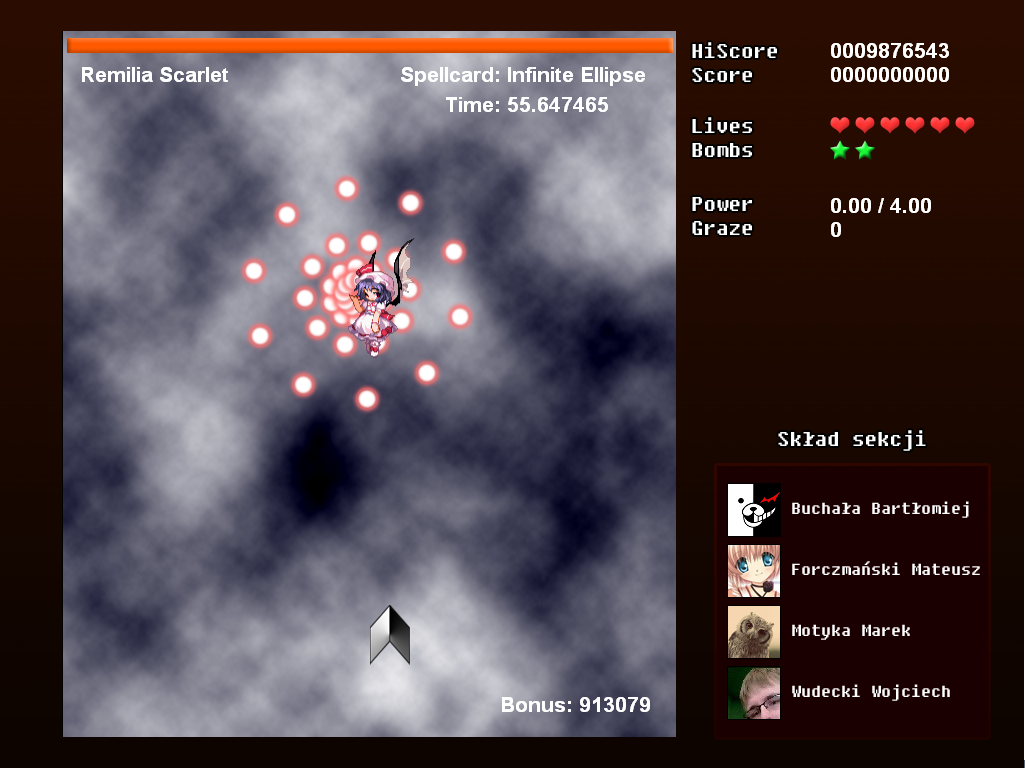
\includegraphics[width=0.70\textwidth]{./images/sz1}
			\end{center}
			Powyższy rysunek prezentuje interfejs gry po jej uruchomieniu. Bomba zostaje uruchomiona, gdy gracz naciśnie przycisk wystrzelenia bomby, domyślnie jest to klawisz X.
			\begin{center}
				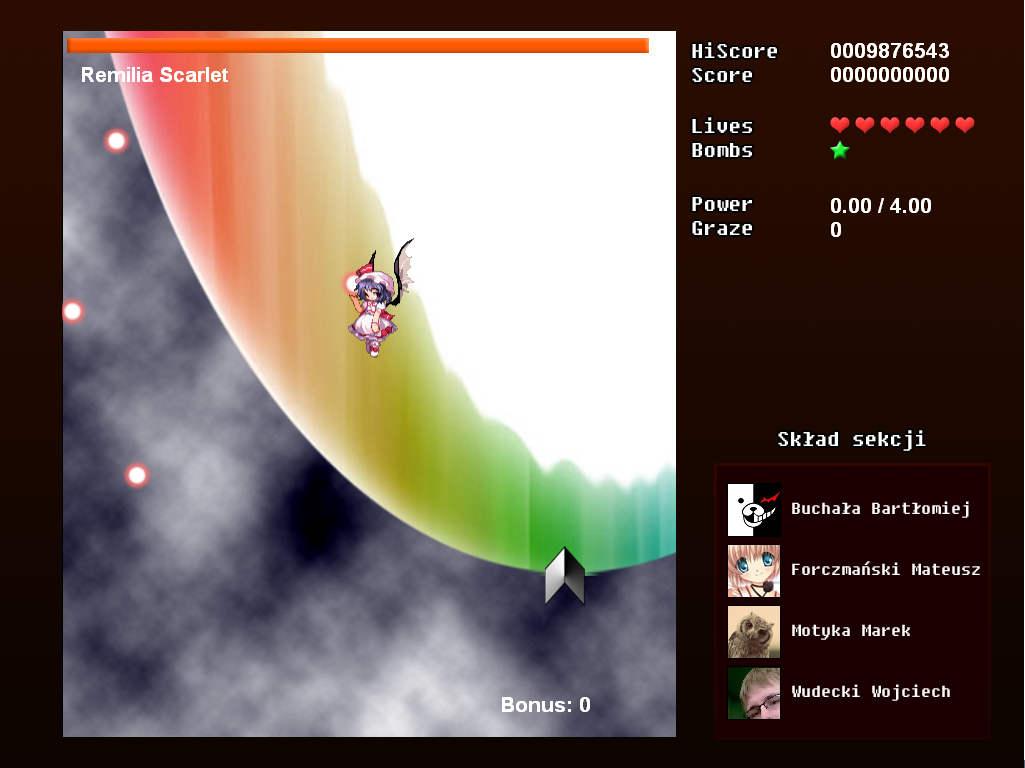
\includegraphics[width=0.70\textwidth]{./images/sz2}
			\end{center}
			Widoczne efekty uruchomienia bomby:
			\begin{itemize}
				\item Narysowanie sprajtu bomby
				\item Dekrementacja licznika, którą można zaobserwować poprzez odjęcie jednej gwiazdki w polu Bombs.
				\item Zmniejszenie paska życia Bossa.
				\item Utrata bonusu za walkę z Bossem.
			\end{itemize}
			
\end{document}